\section{Schema Numerico Semi-Lagrangiano}
\begin{frame}{Strumenti iniziali}
  \begin{itemize}
    \item $S$ superfice regolare chiusa
    \item $\Omega$ dominio limitato in $\mathbb{R}^3$
    \item $\partial\Omega=\{x\in\Omega; u(x)=0\}$ superfice chiusa in form
      level-set, $\partial\Omega$ rappresenta l'\alert{interfaccia} al
      livello zero. 
    \item $\Omega^{-}=\{x\in\Omega; u(x)<0\}$
    \item $\Omega_{+}=\{x\in\Omega; u(x)>0\}$
  \end{itemize}

  \begin{center}
  \tdplotsetmaincoords{60}{40}
  \begin{tikzpicture}[tdplot_main_coords,gray,thick]
    \definecolor{sapC}{rgb}{0.54,0.14,0.14}
    \coordinate (O) at (0.66,0.0,0.0);
       
    \tdplotsetcoord{P}{1.3}{90}{45};
    \tdplotsetcoord{P2}{-2.0}{120}{30};
    \tdplotsetcoord{P3}{3.0}{60}{40};
    \tdplotsetcoord{P4}{0.8}{97}{153};
    \tdplotsetcoord{P5}{1.3}{-55}{40};

    
    \draw [->,sapC](P2) to[out=120,in=180](P5);
    \node[fill=red!15,rotate=50,scale=4.0,rounded corners] at (P4) {};
    \node[shape=circle,draw=gray,fill=gray,inner sep=0pt,minimum size=1mm]
    (origin) at (O) {};
    \node [left,sapC] at (origin.south) {$O$};
    \node[] (end) at (P3) {};
    \node [sapC] at (end.south) {$\Omega^+$};
    \node[] (end1) at (P) {};
    \node [sapC] at (end1.south) {$\Omega^-$};
    \node[] (end2) at (P2) {};
    \node [sapC] at (end2.north) {$\partial\Omega$};

    \draw  [tdplot_main_coords,dashed] (O) ellipse (42pt and 20pt);
    \tdplotsetthetaplanecoords{40};
    \draw [thick,tdplot_rotated_coords](1.0,0.5,0.5) arc (0:360:1.5);
    
        
  \end{tikzpicture}
 \end{center}
\end{frame}

\begin{frame}{Riscriviamo l'integrale nel termine del trasporto}
     L'integrale
    $\iint_{\partial\Omega}\Div\left(\frac{Du}{|Du|}\right)d\mu$ lo
    possiamo riscrivere come per $Du\neq 0$
    \[
    \int_{\Omega}\Div\left(\frac{Du}{|Du|}\right)|Du|\delta(u)dx
    \]
    \begin{itemize}
    \item L'integrale di superfice di una funzione $f(x)$ si può
      definire anche come 
      \[
      \int_{\Omega}f(x)\hat{\delta}(x)dx
      \]   
    \item $\hat{\delta}(x)=DH(u(x))\cdot\mathcal{V}$ delta
      multidimensionale con $\mathcal{V}$ normale esterna ed 
      \[
      H(u(x))=
      \begin{cases}
        0 &\text{ se }u\leq 0 \\
        1 &\text{ se }u > 0
      \end{cases}
      \]
    \item $\hat{\delta}(x)=H'(u(x))Du\cdot\frac{Du}{|Du|}=\delta(u)|Du|$
    \end{itemize}
 \end{frame}

\begin{frame}{Riscriviamo il termine MCM}
  Ricordiamo il flusso MCM essere $tr(P(Du)D^2u)$ con
  $P(Du)=I-\frac{Du\otimes Du}{|Du|^2}$
  \begin{enumerate}
    \item $P(Du)$ matrice di proiezione sul piano tangente alla
      superfice, di rango $2$ con due autovettori relativi
      all'autovalore $\lambda=1$ 
    \item  $v_1$ e $v_2$ autovettori ortonormali di $P$ 
      \[
      v_1=
      \begin{bmatrix}
        \frac{-u_{x_3}}{\sqrt{u_{x_1}^2+u_{x_3}^2}} \\
        0 \\
        \frac{u_{x_1}}{\sqrt{u_{x_1}^2+u_{x_3}^2}}
      \end{bmatrix}
      \quad
      v_2=\frac{1}{|Du|}
      \begin{bmatrix}
        \frac{-u_{x_1}u_{x_2}}{\sqrt{u_{x_1}^2+u_{x_3}^2}} \\
        \sqrt{u_{x_1}^2+u_{x_3}^2} \\
        \frac{-u_{x_2}u_{x_3}}{\sqrt{u_{x_1}^2+u_{x_3}^2}}
      \end{bmatrix}
      \]
    \item per $v_1$ e $v_2$ si verifica che 
    \[
    P(Du)=\sum_{i=1}^2v_i\otimes v_i=\sigma\sigma^t\quad\text{con }
    \sigma=[v_1,v_2]\in\mathbb{R}^{3\times 2} 
    \]
  \end{enumerate}
\end{frame}

\begin{frame}{Riscriviamo il flusso MCM}
  \begin{alertblock}{Flusso MCM}
    Vale la seguente uguaglianza
    \[
    F_{\text{MCM}}(Du,D^2u)=v_1^tD^2uv_1+v_2^tD^2uv_2
    \]
  \end{alertblock}
  \begin{block}{Esplicitazione del conto}
  Sostituiamo l'espressione  $P(p)=\sum_{i=1}^2v_i\otimes
  v_i=\sum_{i=1}^2v_iv_i^t$ nel flusso MCM, ottenendo
  \[
  \begin{aligned}
    tr(P(Du)D^2u)&=tr((v_1v_1^t+v_2v_2^t)D^2u)=\\
    &tr((v_1v_1^t)D^2u+(v_2v_2^t)D^2u).
  \end{aligned}
  \]
  Traccia opertatore lineare
  \[
  \begin{aligned}
    F_{\text{MCM}}(Du,D^2u)&=tr((v_1v_1^t)D^2u)+tr(v_2v_2^t)D^2u)=\\
    &v_1^tD^2uv_1+v_2^tD^2uv_2.
  \end{aligned}
    \]
  \end{block}
\end{frame}

\begin{frame}{Schema Semi-Lagrangiano VPMCM}
  \begin{block}{Griglia spaziale e temporale}
    \begin{itemize}
      \item $x_j=(j_1\Delta x,j_2\Delta x,j_3\Delta x)$,
        $j\in\mathbb{Z}^3$ e $t^n=n\Delta t$, $n\in\mathbb{N}$
      \item $(x_j,t^n)$ punto della griglia $G_{\Delta x}\times
        G^{\Delta t}$
      \item $u_j^n$ approssimazione di $u(x_j,t^n)$
      \item $D_j^n$ approssimazione di $Du(x_j,t^n)$
    \end{itemize}
    \end{block}
  \begin{osservazione}
    I vettori $v_1$ e $v_2$ non sono definiti quando $|Du|=0$ o
    $u_{x_1}^2+u_{x_3}^2=0$. Numericamente introduciamo una soglia:
    \begin{itemize}
    \item \alert{sopra la soglia}
      \[
      |D_j^n|>C\Delta x \land (D_j^n)_1^2+(D_j^n)_3^2>C\Delta x
      \]
    \item \alert{sotto la soglia}
      \[
      |D_j^n|\leq C\Delta x \lor (D_j^n)_1^2+(D_j^n)_3^2\leq C\Delta x
      \]
      \end{itemize}
    \end{osservazione}
\end{frame}

\begin{frame}{Schema Semi-Lagrangiano VPMCM}
  \begin{block}{Equazione di partenza}
    \[
    u_t=v_1^tD^2uv_1+v_2^tD^2uv_2 - \frac{\int_{\Omega}F_{\text{MCM}}(Du,D^2u)\delta(u)dx}{3V_0}x^tDu
    \]
  \end{block}
  \begin{block}{Punti principali della costruzione}
    \begin{enumerate}
    \item Approssimazione flusso VPMCM sopra la soglia
    \item Schema \emph{ad hoc} nel caso sotto la soglia
    \item Approssimazione del coefficente del trasporto $\mathcal{I}$
      al tempo $t$ 
    \end{enumerate}
  \end{block}
\end{frame}
 
\begin{frame}{Approssimazione flusso VPMCM. Caso sopra la soglia}
  \only<1>{\begin{alertblock}{Flusso VPMCM}
    $F_{\text{VPMCM}}=v_1^tD^2uv_1+v_2^tD^2uv_2 -
    \mathcal{I}(u,t)x^tDu$
    \end{alertblock}
  \begin{itemize}
    \item $\mathcal{I}^n$ opportuna approssimazione del coefficente
      del trasporto al  tempo $t^n$
    \item Differenze finite centrare di passo $\Delta x$ 
      \[
      Du\simeq D_j^n\quad v_1(D_j^n)=v_{j,1}^n\quad v_2(D_j^n)=v_{j,2}^n
      \]
    \item \alert{Flusso MCM}: discretizziamo usando incrementi direzionali
      nelle \alert{quattro} direzioni $(\pm v_1\pm v_2)$ con passo
      $\sqrt{2\Delta t}=\rho$
      \[
      \begin{aligned}
        &F_{\text{MCM}}(Du,D^2u)\simeq\frac{1}{2\rho^2}(u(x_j+\rho(v_1+v_2),t)+u(x_j+\rho(v_1-v_2),t)+\\ 
        &u(x_j+\rho(-v_1+v_2),t)+u(x_j+\rho(-v_1-v_2))-4u_j^n).
      \end{aligned}
      \]
  \end{itemize}}
      \only<2>{
        Serie di Taylor nella direzione $v_1+v_2$ 
          \[
          \begin{aligned}
            &u(x+\sqrt{2\Delta t}(v_1+v_2),t^n)=u(x,t^n)+\\
            &<Du(x,t^n),(v_1+v_2)>\sqrt{2\Delta t}+\Delta
            t<D^2u(x_j,t^n)(v_1+v_2),(v_1+v_2)>+\\
            &+T_3\Delta^{\frac{3}{2}} +O(\Delta t^2)
          \end{aligned}
          \]
          Sviluppando nelle altre direzioni e sommando riusciamo ad
          approssimare il flusso con un errore dell'ordine
          $O(\Delta t^2)$.
          \[
          v_1^tD^2uv_1+v_2^tD^2uv_2 =\frac{1}{4\Delta t}(\sum_{+,-}
          u(x_j+\sqrt{2\Delta t}(\pm v_1 \pm
          v_2),t^n)-4u(x,t))+O(\Delta t^2)
          \]
      }

       \only<3>{ 
         \begin{itemize}
           \item Incrementi nelle \alert{quattro} direzioni $(\pm
         v_1\pm v_2)$ più ci andiamo a ricostruire la parte di
         trasporto indietro lungo la caratteristica
         \[
         \begin{aligned}
           &F_{\text{VPMCM}}\simeq\frac{1}{4\Delta
          t}(u(x_j(1-\mathcal{I}^n\Delta t)+\sqrt{2\Delta
             t}(v_{j,1}^n+v_{j,2}^n),t)+ \\
           &u(x_j(1-\mathcal{I}^n\Delta t)+\sqrt{2\Delta
             t}(v_{j,1}^n-v_{j,2}^n),t)+\\
           &u(x_j(1-\mathcal{I}^n\Delta t)+\sqrt{2\Delta
             t}(-v_{j,1}^n+v_{j,2}^n),t)+\\
           &u(x_j(1-\mathcal{I}^n\Delta t)+\sqrt{2\Delta
             t}(-v_{j,1}^n-v_{j,2}^n),t)-4u_j^n)
         \end{aligned}
         \]
       \end{itemize}}
\end{frame}

\begin{frame}{Schema SL VPMCM sopra la soglia}
  \begin{alertblock}{VPMCM \emph{fully discrete}}
    \begin{itemize}
    \item Approssimazione coefficente del trasporto $\mathcal{I}^n$
    \item Differenze finite centrate per $D_j^n$ più
      $v_i(D_j^n)=v_{j,i}^n$
    \item Approssimazione del flusso $F_{VPMCM}$
    \item Differenze finite in avanti per
      $u_t\simeq\frac{u(x_j,t^{n+1})-u(x_j,t^n)}{\Delta t}$
    \item Interpolazione lineare $I[\cdot]$ nei punti
      $x_j(1-\mathcal{I}^n\Delta t)+\sqrt{2\Delta t}(\pm
      v_{j,1}^n\pm v_{j,2}^n)$
    \end{itemize}
    \[
    \begin{aligned}
        u_j^{n+1}&=\frac{1}{4}(I[u^n](x_j(1-\mathcal{I}^n\Delta t)+\sqrt{2\Delta
          t}(v_{j,1}^n+v_{j,2}^n))+ \\
        &I[u^n](x_j(1-\mathcal{I}^n\Delta t)+\sqrt{2\Delta
          t}(v_{j,1}^n-v_{j,2}^n))+\\
        &I[u^n](x_j(1-\mathcal{I}^n\Delta t)+\sqrt{2\Delta
          t}(-v_{j,1}^n+v_{j,2}^n))+\\
        &I[u^n](x_j(1-\mathcal{I}^n\Delta t)+\sqrt{2\Delta
          t}(-v_{j,1}^n-v_{j,2}^n))
    \end{aligned}
    \]
  \end{alertblock}
\end{frame}
 
\begin{frame}{Approssimazione flusso VPMCM. Caso sotto la soglia}
  Nel caso sotto la soglia $|D_j^n|\leq C\Delta x$ o
  $(D_j^n)_1^2+(D_j^n)_3^2\leq C\Delta x$, 
  \[
  u_j^{n+1}=\frac{1}{6}\sum_{i\in D(j)}u_i^n
  \]
con $D(j)=\{j\pm e_i\Delta x\,,i=1,2,3\}$, che rappresenta
l'approssimazione dell'equazione del calore
\[
u_t=\varepsilon \Delta u,\quad \varepsilon=\frac{\Delta x^2}{6\Delta t}
\]
Questo metodo è lo stesso utilizzato nello schema classico MCM e 
risulta consistente con $\underline{F}(Du,D^2u)$ e
$\overline{F}(Du,D^2u)$ suggerite da \emph{Crandall and Lions}.
\[
\underline{F}=
\begin{cases}
-\Div\left(\frac{Du}{|Du|}\right)|Du| &\text{ se }Du\neq 0\\
-2||D^2u|| &\text{ se }Du=0
\end{cases}\,\,
\overline{F}=
\begin{cases}
-\Div\left(\frac{Du}{|Du|}\right)|Du| &\text{ se }Du\neq 0\\
2||D^2u|| &\text{ se }Du=0
\end{cases}
\]
\end{frame}

\begin{frame}{Approssimazione dell'integrale}
  Integrale $\mathcal{I}(u,t)=\int_{\Omega}F_{\text{MCM}}(Du,D^2u)\delta(u)dx$
  \begin{itemize}
    \item delta: usiamo la derivata della funzione
      \emph{smeared-out} di Heaviside con $\varepsilon=1.5\Delta x$
      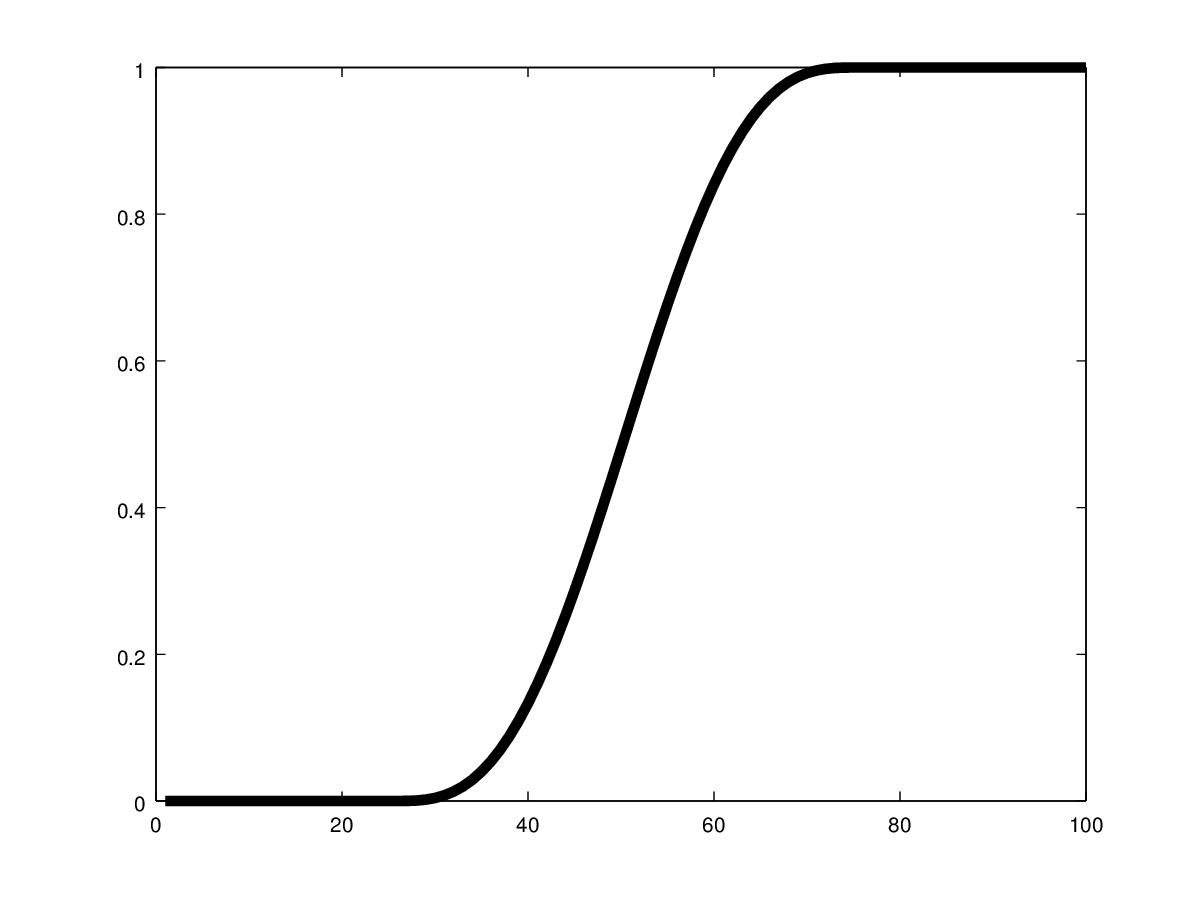
\includegraphics[width=0.3\textwidth]{graphics/heavside/heavside}
        \item Formula del punto medio Composita
          \[
          \mathcal{I}^n=\frac{1}{3V_0}\Delta x^3\sum_{j=1}^{|G_{\Delta x}|}F_j^n\tilde{\delta}(u_j^n)
          \]
  \end{itemize}
\end{frame}


\begin{frame}{Flusso VPMCM nel caso della sfera}
  \begin{columns}[T]
    \begin{column}{6.5cm}
      \begin{exampleblock}{Caso semplificato, evoluzione della sfera}
        $S(R(t))$ famiglia di sfera in forma level-set
        \begin{itemize}
        \item $S_0=\{x\in\mathbb{R}^3| |x|^2-R_0^2=0\}$
        \item $V(R(t))=V_0\Rightarrow R(t)=R_0$
        \item $\mathcal{I}(\mathcal{H}(u),t)=2\frac{4\pi}{3V_0}R_0=2\left(\frac{4\pi}{3V_0}\right)^\frac{2}{3}$.
        \end{itemize}
      \end{exampleblock}
    \end{column}
    \begin{column}[T]{3.5cm}
      \begin{center}
        \only<2->{\animategraphics[autoplay,loop,width=1.0\textwidth,height=0.45\textheight]{0.8}{smooth/vpmcm/sphere/sphere}{0}{4}}
      \end{center}
  \end{column}
\end{columns}
\end{frame}

\begin{frame}{Consistenza generalizzata}
  \begin{definizione}[Consistenza]
    Sia $\phi\in C^{\infty}(\mathbb{R}^3\times[0,T])$ e $(\Delta
    x_m,\Delta t_m)\to (x,t)$ e  $(x_{n_m},t^{n_m})\to 0$  per
    $m\to\infty$, con $(\Delta x_m,\Delta t_m)$  seguenza di
    parametri di discretizzazione e $(x_{j_m},t^{n_m})$ seguenza di
    nodi. Allora lo schema $S$ è consistente con
    \[
    \phi_t(x,t)+F(x,D\phi,D^2\phi)=0
    \]
    se
    \[
    \left\{
    \begin{aligned}
      &\liminf_{m\to\infty}\frac{\phi(x_j,t_{n_m+1})-S_{j_m}(\phi^{n_m})}{\Delta
        t_m}\geq\phi_t(x,t)+F_*(x,D\phi,D^2\phi)
        \\
       &\limsup_{m\to\infty}\frac{\phi(x_j,t_{n_m+1})-S_{j_m}(\phi^{n_m})}{\Delta
          t_m}\leq\phi_t(x,t)+F^*(x,D\phi,D^2\phi)
    \end{aligned}
    \right.
    \]
    con $F_*$ inviluppo semicontinuo inferiore e $F^*$ inviluppo
    semicontinuo superiore.
  \end{definizione}
\end{frame}

\begin{frame}{Consistenza caso sfera con $Du\neq 0$}
  \begin{alertblock}{Schema sopra la soglia per la sfera}
   \[
     u_j^{n+1}=\frac{1}{4}\sum_{+,-}(I[u^n](x_j(1-C\Delta
     t)+\sqrt{2\Delta t}(\pm v_{j,1}^n\pm v_{j,2}^n))
    \]
    con $C=2\left(\frac{4\pi}{3V_0}\right)^\frac{2}{3}$.
  \end{alertblock}
  Supponiamo
  \begin{itemize}
    \item $u$ sufficentemente regolare
    \item $||I[u^n](\cdot)-u(\cdot,t^n)||=O(\Delta x^2)$ errore di
      interpolazione 
    \item $|D_j^n-Du(x_j,t^n)|=O(\Delta x^2)$ errore approssimazione
      del gradiente
   \end{itemize}
  Osserviamo \\ 
      $|J_{\sigma}(p)|=\frac{1}{p_1^2+p_3^2}$ con $p=Du$ e
      $\sigma=[v_1,v_2]$ matrice $3\times 2$,  poichè vale
      $(D_j^n)_1^2+(D_j^n)_3^2\geq C\Delta x$ allora $\sigma$ è
      lipschitiziana con $L_{\sigma_j^n}=\frac{1}{C\Delta x}$.  
 \end{frame}

\begin{frame}{Consistenza caso $Du\neq 0$}
Iniziamo la stima per \alert{$v_1+v_2=\sigma(D_j^n)b$} con $b=[1,1]^t$
\[
\begin{aligned}
  &I[u^n](x_j-x_jC\Delta t +\sqrt{2\Delta t}\sigma(D_j^n)b,t^n)=\\
  &u(x_j-x_jC\Delta t +\sqrt{2\Delta t}\sigma(Du(x_j,t^n))b,t^n)+\\
  &O(\Delta x^2) + O(\Delta x\Delta t^{\frac{1}{2}}) 
\end{aligned}
\]
Espansione di Taylor del terzo ordine otteniamo
\[
\begin{aligned}
&u(x_j-x_jC\Delta t +\sqrt{2\Delta
    t}(v_1+v_2),t^n)=u(x_j,t^n)+\\
&<Du(x_j,t^n),(v_1+v_2)>\sqrt{2\Delta t}+\Delta
  t<D^2u(x_j,t^n)(v_1+v_2),(v_1+v_2)>+\\
&-C<Du(x_j,t^n),x_j>\Delta t+T_3\Delta^{\frac{3}{2}} +O(\Delta t^2)
\end{aligned}
\]
Ripetendo il calcolo per $(\pm v_1\pm v_2)$ e sommando abbiamo
\[
\begin{aligned}
S_j(u^n)&=u(x_j,t^n)+\Delta t(v_1^tD^2u(x_j,t^n)v_1+v_2^tD^2u(x_j,t^n)v_2-Cx^tDu(x_j,t^n))+\\
&O(\Delta x^2)+ O(\Delta x\Delta t^{\frac{1}{2}})+ O(\Delta t^2)
\end{aligned}
\]
\end{frame}

\begin{frame}{Consistenza caso $Du\neq 0$}
In conclusione utilizziamo la definizione di consistenza generalizzata
\[
\begin{aligned}
\frac{u(x_j,t^{n+1})-S_j(u^n)}{\Delta
  t}&=u_t(x_j,t^n)-v_1^tD^2u(x_j,t^n)v_1-v_2D^2u(x_j,t^n)v_2+\\
& Cx^tDu(x_j,t^n)+O(\Delta x^2\Delta t^{-1})+O(\Delta x\Delta
t^{-\frac{1}{2}})+O(\Delta t)
\end{aligned}
\]
\begin{alertblock}{Conclusione}
Poniamo ad esempio $\Delta t=\Delta x^{\alpha}$, affinchè il metodo
sia consistente per $(\Delta x,\Delta t)\to 0$ e $(x_j,t^n)\to (x,j)$
abbiamo 
\[
\begin{aligned}
&L_{\Delta x}\simeq\Delta x^{2-\alpha}+\Delta
x^{1-\frac{\alpha}{2}}+\Delta x \\
&\Delta x^{2-\alpha}\to 0\land\Delta x^{1-\frac{\alpha}{2}}\to 0\Rightarrow0<\alpha<2
\end{aligned}
\]
Quindi il metodo non richiede una CFL parabolica, per la quale
$\Delta t=O(\Delta x^2)$.
\end{alertblock}
\end{frame}

